\section{Theorie}
\label{sec:Theorie}

Experimentelle Untersuchungen zeigen, dass Licht nur durch die Quantenelektrodynamik widerspruchsfrei beschrieben werden.
Für eine große Zahl von Photonen, den sogenannten Feldquanten der Elektrodynamik,
kann die räumliche Ausbreitung des Lichtes durch das Wellenmodell genähert, wie es zum Beispiel in der Beugungsoptik geschieht. 

Bei Wechselwirkungen zwischen Licht und Materie, wie es bei dem Photoeffekt der Fall ist, 
stellt das Korpuskelmodell eine bessere Beschreibung des Phänomens dar, welches im Folgenden behandelt wird.
 

\subsection{Die Phänomene und Erklärung des Photoeffektes nach der Einsteinschen Korpuskulartheorie}

Wird eine Metalloberfläche mit Photonen der Energie
\begin{equation}
    E_\text{photon} = h \nu     \label{eq:photonenenergie}
\end{equation}
bestrahlt, können durch diese Elektronen aus dem Metall herausgelöst werden. 
Das Photon überträgt dabei seine Energie dem sich im Metall befindlichen Elektron. 
Zum Verlassen des Metalls muss die spezifische Austrittsarbeit der Kathode $\Phi_\text{K}$ geleistet werden.
Die verbleibende Energie wird in die kinetische Energie $E_\text{kin} \geq 0 \,$ des Elektrons umgesetzt. 
Die Energiebilanz für ruhende Elektronen (vgl. Abschnitt 2.2 für bewegte Elektronen) lautet demnach
\begin{equation}
    h \nu = \Phi_\text{K} + E_\text{kin} \, .    \label{eq:bilanz_elektron} 
\end{equation}

Demnach ist die Energie $E_\text{kin}$ der Elektronen nach dem Stoß proportional zur Lichtfrequenz $\nu$.
Der Photoeffekt tritt nur auf wenn, $h \nu < \Phi_\text{K}$ gilt.
Es existiert also eine minimale Grenzfrequenz unterhalb derer keine Elektronen mehr aus dem Metall gelöst werden können.
Des Weiteren ist zu beobachten, dass die Anzahl der ausgelösten Elektronen proportional zur Intensität des Lichtes ist.


\subsection{Experimenteller Nachweis des Photoeffektes} \label{sec:nachweis}

Der Nachweis des photoelektrischen Effektes geschieht durch eine Messung der ausgelösten Elektronen.
In \autoref{fig:photoeffekt} ist der prinzipieller Aufbau der Messung dargestellt,
dabei wird eine positiv geladene Auffängerelektrode einer Photokathode gegenübergestellt.
Dieses Konzept wird mithilfe einer Photozelle in \autoref{fig:photozelle} realisiert.
\begin{figure}
    \begin{subfigure}{0.48\textwidth}
        \centering
        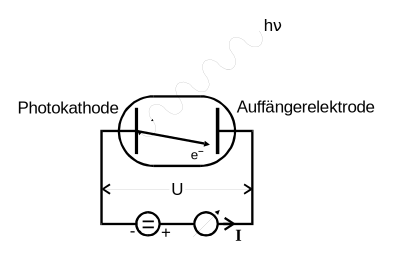
\includegraphics[height=5cm]{bilder/photoeffekt_schema.pdf}
        \caption{Schematischer Versuchsaufbau. \cite{v500}}
        \label{fig:photoeffekt}
    \end{subfigure}
    \hfill
    \begin{subfigure}{0.48\textwidth}
        \centering
        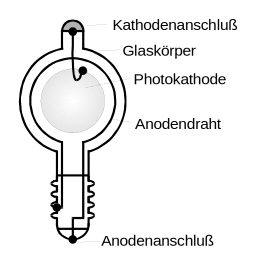
\includegraphics[height=5cm]{bilder/photozelle_aufbau.pdf}
        \caption{Aufbau der Photozelle. \cite{v500}}
        \label{fig:photozelle}
    \end{subfigure}
\end{figure}

Wenn ein Elektron von der Photokathode auf die Auffängerelektrode trifft, wird dein Strom gemessen.
Die Kathode besteht dabei aus einer dünnen Metallschicht im Inneren der Photozelle.
Die Anode ist durch einen Drahtring wenige Millimeter vor der Kathode realisiert. 
Um Störeffekte mit Gasmolekülen zu vermeiden, ist das Innere des Glaskolben weitgehend evakuiert.

Zwischen Kathode und Anode wird ein elektrisches Bremsfeld erzeugt, 
indem eine variable Spannungsquelle angeschlossen wird. 
Zur Messung der ausgelösten Elektronen wird ein Picoamperemeter verwendet.
Die elektrische Schaltung ist in \autoref{fig:schaltbild} dargestellt.
\begin{figure}
    \centering
    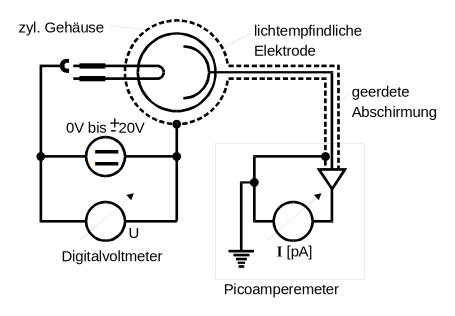
\includegraphics[width=0.6\textwidth]{bilder/schaltbild.pdf}
    \caption{Schaltbild der Messapparatur. \cite{v500}}
    \label{fig:schaltbild}
\end{figure}

Durch das Bremsfeld mit der Spannung $U_\text{B}$ können nur Elektronen mit
$E_\text{kin} > e_0 U_\text{B} $ die Auffängerelektrode erreichen. 
Für die Grenzspannung
\begin{equation}
    e_{0} U_\text{g} = \frac{1}{2} m_{0} v_\text{max}^{2}  \label{eq:grenzspannung}
\end{equation}
verschwindet der gemessene Strom, da selbst die Energie der schnellsten Elektronen nicht
ausreicht, um die Elektrode zu erreichen. 
Nach \autoref{eq:bilanz_elektron} gilt für diese Elektronen
\begin{equation}
    h \nu = \Phi_\text{K} + e_{0} U_\text{g} \, .   \label{eq:schnellste_elektronen} 
\end{equation}

Elektronen mit der Geschwindigkeit $v < v_\text{max}$ erreichen schon für eine Spannung
$U_\text{B} < U_\text{g}$ nicht mehr die Elektrode. 
Deswegen sinkt der gemessene Photostrom kontinuierlich ab, bis er bei $U_\text{g}$ Null erreicht. 
Dies ist in \autoref{fig:photostrom} abgebildet.
\begin{figure}
    \centering
    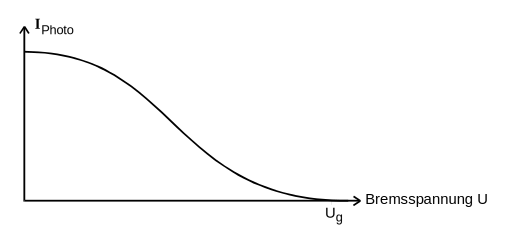
\includegraphics[width=0.7\textwidth]{bilder/photostrom.pdf}
    \caption{Photostrom in Abhängigkeit der Bremsspannung. \cite{v500}}
    \label{fig:photostrom}
\end{figure}

Die Energie der ausgelösten Photoelektronen hängt von der bereits in dem Festkörper vorhandenen kinetischen Energie der Elektronen ab.
Diese unterschiedliche Energieverteilung vefolgt die $\textit{Fermi-Dirac-Statistik}$, welche besagt,
dass sich die Energie der Leitungs- und Valenzelektronen von 0 biszur Fermi-Enerie $\zeta$ erstreckt, 
wobei $\zeta$ materialabhängig ist.

Unter bestimmten Voraussetzungen besteht zwischen dem gemessenen Photostrom $I_\text{Ph}$
und der Bremsspannung $U_\text{B}$ der Zusammenhang
\begin{equation*}
    I_\text{Ph} \propto U_\text{B} \, .
\end{equation*}

Des Weiteren kann der Fall eintreten, dass zwar $\Phi_\text{K} < h \nu$ gilt, 
also Elektronen aus der Kathode gelöst werden, 
aber für die Austrittsarbeit der Anode $\Phi_\text{A} > h \nu$ gilt, 
sodass kein Strom an der Anode gemessen (siehe \autoref{fig:fermi1}).
Dies liegt an dem elektrischen Gegenfeld, welches durch die Differenz der
Fermi-Niveaus von Kathode und Anode entsteht und die Elektronen so stark abbremst, 
dass sie die Anode nicht mehr erreichen.
Nach Anlegen eines beschleunigenden Potentials $U_\text{b}$ in \autoref{fig:fermi2}
kann jedoch wieder ein Photostrom gemessen werden, sodass gilt
\begin{equation}
    h \nu + e_{0} U_\text{B} \geq \Phi_\text{A} \, .    \label{eq:beschleunigendes_Potential}
\end{equation}

\begin{figure}
    \begin{subfigure}{0.48\textwidth}
        \centering
        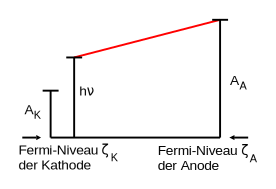
\includegraphics[height=5cm]{bilder/fermi1.pdf}
        \caption{Potentialdifferenz zwischen Anode und Kathode. \cite{v500}}
        \label{fig:fermi1}
    \end{subfigure}
    \hfill
    \begin{subfigure}{0.48\textwidth}
        \centering
        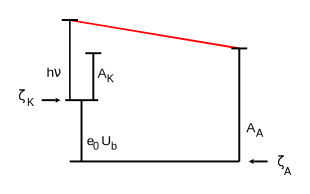
\includegraphics[height=5cm]{bilder/fermi2.pdf}
        \caption{Anlegen eines beschleunigenden Potentials $U_\text{B}$ zur Erzeugung eines Photostroms. \cite{v500}}
        \label{fig:fermi2}
    \end{subfigure}
\end{figure}